\section{Длина окружности и её частей}

\paragraph{Предварительное разъяснение.}\label{1938/226}
Отрезок можно сравнить с другим отрезком, принятым за единицу, так как прямые линии при наложении совмещаются.
Действительно, только по этой причине мы можем установить, какие отрезки считать равными и неравными;
что такое сумма отрезков или какой отрезок более другого в $2, 3, 4,\dots$ раза.
Точно так же дуги окружностей одинакового радиуса можно сравнить между собой вследствие того, что такие дуги при наложении совмещаются.
Но так как никакая часть окружности (или другой кривой) не может совместиться с прямой, то нельзя путём наложения установить, какой криволинейный отрезок должно считать равным данному прямолинейному отрезку, а следовательно, и то, какой криволинейный отрезок больше данного прямолинейного в $2,3,4,\dots$
раза.
Таким образом, является необходимость особо определить, что мы будем подразумевать под длиной окружности (или части её), когда сравниваем её с прямолинейным отрезком.

Для этой цели мы должны ввести новое понятие, имеющее исключительно большое значение во всей математике, именно понятие о пределе.

\subsection*{Пределы}

\paragraph{Предел числовой последовательности.}\label{1938/227}
Во многих вопросах алгебры и геометрии приходится встречаться с последовательностями чисел, написанных одно за другим по определённому закону.
Например, натуральный ряд чисел:
\[1, 2, 3, 4, 5,\dots,\]
арифметическая и геометрическая прогрессии, продолженные неограниченно:
\[a,a+d,a+2d,a+3d,\dots,\]
\[a,aq,aq^2,aq^3,\dots,\]
представляют собой бесконечные последовательности чисел или бесконечные числовые последовательности.

Для каждой такой последовательности можно указать правило, по которому составляются её члены.
Так, в арифметической прогрессии каждый член разнится от предыдущего на одно и то же число, в геометрической прогрессии каждый член равен предшествующему, умноженному на некоторое определённое число (знаменатель прогрессии).

Многие последовательности составляются по более сложным правилам.
Так, например, вычисляя $\sqrt{2}$ с недостатком, сначала с точностью до $\tfrac1{10}$, затем с точностью до $\tfrac1{100}$, затем до $\tfrac1{100}$ и продолжая это вычисление неограниченно, мы получим бесконечную числовую последовательность:
\[1{,}4;
1{,}41;
1{,}414;
1{,}4142,\dots,\]
дающую приближённое значение  $\sqrt{2}$  с возрастающей степенью точности.

Для этой последовательности нельзя указать простого правила, по которому можно было бы получить новые её члены, зная предыдущие, но все же можно определить любой член этой последовательности.
Так, чтобы получить 4-й её член, нужно вычислить с точностью до $0{,}0001$, для получения 5-го члена нужно вычислить  $\sqrt{2}$  с точностью до $0{,}00001$ и~т.~д.

Допустим, что члены данной бесконечной последовательности $a_1$, $a_2$, $a_3, \dots, a_n,\dots$ по мере повышения их номера неограниченно приближаются к некоторому числу $A$.
Это значит следующее:
существует некоторое число $A$, такое, что какое бы малое положительное число $q$ мы ни взяли, в данной последовательности можно отыскать член, начиная с которого все члены последовательности по абсолютной величине отличаются от $A$ меньше, чем на $q$.
Мы будем это свойство коротко выражать так:
 абсолютная величина разности $a_n-A$
неограниченно убывает с возрастанием номера $n$.

В этом случае число $A$ называется \rindex{предел}\textbf{пределом} данной бесконечной числовой последовательности.
Приведём пример такой последовательности.
Составим последовательность десятичных дробей.
\[0{,}9;
0{,}99;
0{,}999;\dots,\]
Здесь каждый член получается из предыдущего приписыванием нового десятичного знака 9.

Легко заметить, что члены этой последовательности неограниченно приближаются к единице.

Именно, первый член отличается от единицы на $\tfrac1{10}$, 
второй на $\tfrac1{100}$, третий на $\tfrac1{1000}$ и, если достаточно продолжить эту последовательность, то можно найти в ней член, начиная с которого все последующие члены будут отличаться от единицы на сколь угодно малую, заранее указанную величину.
Следовательно, мы можем сказать, что взятая нами бесконечная числовая последовательность имеет пределом единицу.

Другим примером числовой последовательности, имеющей предел, служит последовательность приближённых значений длины отрезка, несоизмеримого с единицей длины (§~\ref{1938/150}), вычисленных с недостатком, сначала с точностью до $\tfrac1{10}$, затем $\tfrac1{100}$, затем — до $\tfrac1{1000}$ и~т.~д.

Пределом этой последовательности служит бесконечная десятичная дробь, представляющая точную меру длины данного отрезка.
В самом деле, величина бесконечной десятичной дроби заключена между двумя её приближёнными значениями, вычисленными с одинаковой точностью — одно с недостатком, другое с избытком. 
Как было показано выше, эта разность неограниченно убывает по мере повышения степени точности приближённых значений.
Следовательно, должна неограниченно убывать и разность между самой бесконечной десятичной дробью и её приближёнными значениями по мере повышения степени точности этих значений.
Значит, бесконечная десятичная дробь служит пределом последовательности всех её приближённых значений, взятых с недостатком (или всех приближённых значений, взятых с избытком).

Легко заметить, что не всякая бесконечная последовательность имеет предел;
например, натуральный ряд чисел.
\[1, 2, 3, 4, 5,\dots,\]
очевидно, никакого предела не имеет, так как его члены неограниченно возрастают и ни к какому числу не приближаются.

\paragraph{}\label{1938/228}
\so{Теорема}.
\textbf{\emph{Всякая бесконечная числовая последовательность может иметь только один предел.}}

В справедливости этой теоремы легко убедиться доказательством от противного.
В самом деле, предположим, что дана последовательность
\[a_1,a_2,a_3,\dots,a_n,\dots,\]
которая имеет два различных предела $A$ и $B$.
В таком случае, в силу того, что $A$ есть предел данной последовательности, абсолютная величина разности $a_n-A$ должна неограниченно убывать с возрастанием $n$.
В силу того, что $B$ есть тоже предел данной последовательности, абсолютная величина разности $a_n-B$ также должна неограниченно убывать с возрастанием $n$.
Но в таком случае абсолютная величина разности
\[(a_n-A)-(a_n-B)\]
должна также или неограниченно убывать, или быть равной нулю.
Но эта последняя разность равна разности чисел $B-A$ и, следовательно, есть некоторое вполне определённое, отличное от нуля число.
Это число не зависит от номера $n$ и при возрастании $n$ вовсе не изменяется.
Таким образом, предположение, что существуют два предела числовой последовательности, привело нас к противоречию.
{\sloppy 
\paragraph{Предел возрастающей бесконечной числовой последовательности.}\label{1938/229}
Рассмотрим такую последовательность 
\[a_1, a_2, a_3,\dots,a_n,\dots,\]
в которой каждый следующий член больше предыдущего, то есть $a_{n+1} \z> a_n$, и в то же время все члены последовательности меньше некоторого определённого числа $M$, то есть $a_n < M$ для любого номера $n$.

}

В этом случае последовательность имеет определённый предел (теорема Вейерштрасса).

\paragraph{}\label{1938/230}
\so{Доказательство}.
Пусть дана бесконечная числовая последовательность
\[a_1,a_2,a_3,\dots,a_n,\dots,
\eqno(1)\]
в которой каждый член больше предыдущего или равен ему (то есть $a_{n+1}\ge a_n$ для всякого $n$), При этом среди членов последовательности нет числа, большего данного числа $M$, например, нет числа, большего, чем $10$.

Возьмём число $9$ и смотрим, нет ли среди членов последовательности (1) чисел, больше, чем $9$.
Допустим, что таких нет.
Возьмём число $8$ и смотрим, имеются ли в последовательности (1) числа больше, чем $8$.
Допустим, что такие есть.
Тогда записываем число $8$, затем делим промежуток от $8$ до $9$ на $10$ частей и испытываем последовательно числа:
$8{,}1; 8{,}2; 8{,}3;\dots$, то есть смотрим, имеются ли среди членов последовательности (1) числа, б\'{о}льшие, чем $8{,}1$.
Если есть, то ставим тот же вопрос для числа $8{,}2$ и~т.~д.
Допустим, что в последовательности (1) есть числа, б\'{о}льшие, чем $8{,}6$, но нет чисел, б\'{о}льших, чем $8{,}7$.
Тогда делаем вторую запись:
пишем число $8{,}6$, затем разбиваем промежуток от $8{,}6$ до $8{,}7$ на $10$ частей и испытываем таким же образом последовательно числа: $8{,}61; 8{,}62; 8{,}63;\dots$.
Допустим, что в последовательности (1) есть числа, б\'{о}льшие, чем $8{,}64$, но нет чисел, б\'{о}льших, чем $8{,}65$.
Тогда делаем третью запись $8{,}64$ и поступаем таким же образом для промежутка от $8{,}64$ до $8{,}65$.

Продолжая этот процесс неограниченно, мы придём к бесконечной десятичной дроби:
$8{,}64\dots$, то есть
к некоторому вещественному числу.
Назовём его $\alpha$ и возьмём его приближённые значения с $n$ десятичными знаками с недостатком и с избытком (§~\ref{1938/150}).
Первое назовём $\alpha_n$, второе —  $\alpha_n'$.
Эти приближённые значения можно выбрать так, что.
\[\alpha_n< \alpha\le\alpha_n'
\quad\text{и}\quad
\alpha_n'-\alpha_n=\tfrac1{10^n}.\] 
Из способа образования вещественного числа $\alpha$ следует, что среди членов последовательности (1) нет чисел, б\'{о}льших $\alpha_n'$, но имеются числа, б\'{о}льшие $\alpha_n$.
Пусть $a_k$, — одно из таких чисел.
\[\alpha_n< a_k<\alpha_n'.\]
В силу возрастания последовательности (1) и отсутствия в ней членов, б\'{о}льших $\alpha_n'$, заключаем, что все следующие члены последовательности $a_{k+1}$, $a_{k+2}, \dots$ также заключены между $\alpha_n$ и  $\alpha_n'$, то есть
если $m > k$, то 
\[\alpha_n< a_m<\alpha_n'.\]

Так как вещественное число $\alpha$ также заключено между $\alpha_n$ и $\alpha_n'$, то абсолютная величина разности $a_m-\alpha$ меньше разности чисел $\alpha_n'$ и $\alpha_n$.
Но $\alpha_n'-\alpha_n=\tfrac1{10^n}$, следовательно,
\[|a_m-\alpha|<\tfrac1{10^n}.
\eqno(2)\]
Таким образом, для любого значения $n$ можно указать такое число $k$, что при $m \ge k$ к имеет место неравенство (2).
Так как при неограниченном возрастании $n$ дробь $\tfrac1{10^n}$ неограниченно убывает, то из неравенства (2) следует, что вещественное число $\alpha$ есть предел последовательности (1).
Таким образом, числовая последовательность (1) имеет определённый предел.

\subsection*{Длина окружности}

Понятие о пределе даст возможность точно определить, что мы подразумеваем под длиной окружности.
Предварительно докажем следующие леммы.

\paragraph{}\label{1938/232}
\so{Лемма 1}.
\textbf{\emph{Выпуклая ломаная}} ($ABCD$, рис.~\ref{1938/ris-231}) \textbf{\emph{меньше всякой другой ломаной}} ($AEFGD$), \textbf{\emph{объемлющей первую.}}

\begin{wrapfigure}{R}{45mm}
\centering
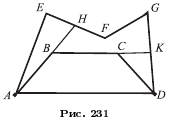
\includegraphics{mppics/ris-231}
\caption{}\label{1938/ris-231}
\end{wrapfigure}


Выражения «объемлющая ломаная», «объемлемая ломаная» имеют следующий смысл.

Пусть две ломаные (как те, которые изображены у нас на рисунке) имеют одни и те же концы $A$ и $D$ и расположены таким образом, что одна ломаная ($ABCD$) вся лежит внутри многоугольника, образованного другой ломаной и отрезком $AD$, соединяющим концы $A$ и $D$;
тогда внешняя ломаная называется объемлющей, а внутренняя ломаная — объемлемой.

Предстоит доказать, что объемлемая ломаная $ABCD$ (если она выпуклая) короче всякой объемлющей линии $AEFGD$ (всё равно — выпуклой или невыпуклой), то есть
что
\[AB+BC+CD<AE+EF+FG+GD.\]
Продолжим стороны выпуклой ломаной так, как указано на рисунке.
Тогда, приняв во внимание, что отрезок меньше всякой ломаной, соединяющей концы отрезка, мы можем написать следующие неравенства.
\[AB+BH<AE+EH;\]
\[BC+CK<BH+HF+FG+GK;\]
\[CD<CK+KD.\]

Сложим почленно все эти неравенства и затем от обеих частей полученного неравенства отнимем вспомогательные отрезки $BH$ и $CK$;
далее, заменив сумму $EH+HF$ отрезком $EF$ и сумму $GK\z+KD$ отрезком $GD$, получим то неравенство, которое требовалось доказать.

\begin{figure}[h!]
\begin{minipage}{.48\textwidth}
\centering
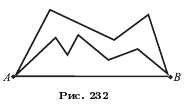
\includegraphics{mppics/ris-232}
\end{minipage}\hfill
\begin{minipage}{.48\textwidth}
\centering
\includegraphics{mppics/ris-233}
\end{minipage}

\medskip

\begin{minipage}{.48\textwidth}
\centering
\caption{}\label{1938/ris-232}
\end{minipage}\hfill
\begin{minipage}{.48\textwidth}
\centering
\caption{}\label{1938/ris-233}
\end{minipage}
\vskip-4mm
\end{figure}

\smallskip
\mbox{\so{Замечание}.}
Если бы объемлемая линия не была выпуклой (рис. \ref{1938/ris-232}), то изложенное доказательство нельзя было бы применить.
В этом случае объемлемая ломаная может оказаться и больше объемлющей.

\paragraph{}\label{1938/233}
\so{Лемма 2}.
\textbf{\emph{Периметр любого выпуклого многоугольника}} ($ABCD$) \textbf{\emph{меньше периметра всякого другого многоугольника}} ($MNPQRL$), \textbf{\emph{объемлющего первый}} (рис.~\ref{1938/ris-233}).


Требуется доказать, что
\[AB+BC+CD+DA < LM+MN+NP+PQ+QR+RL.\]
Продолжив в обоих направлениях сторону $AB$ выпуклого многоугольника, применим к ломаным линиям $ABCD$ и $ATMNPQRSD$, соединяющим точки $A$ и $B$, лемму предыдущего параграфа;
получим неравенство:
\[AB+BC+CD<AT+TM+MN+NP+PQ+QR+RS+SD.\]
С другой стороны, так как отрезок $ST$ меньше ломаной $SLT$, то можем написать:
\[TA+AD+DS<TL+SL.\]
Сложим почленно эти два неравенства и отнимем от обеих частей вспомогательные отрезки $AT$ и $DS$;
далее, заменив сумму $TL+TM$ отрезком $LM$ и сумму $LS+RS$ отрезком $LR$, получим то, что требовалось доказать.

\begin{wrapfigure}{r}{30mm}
\centering
\includegraphics{mppics/ris-234}
\caption{}\label{1938/ris-234}
\end{wrapfigure}

\paragraph{Определение длины окружности.}\label{1938/234}
Впишем в данную окружность (рис.~\ref{1938/ris-234}) правильный многоугольник, например треугольник, и на какой-нибудь прямой $MN$ (рис.~\ref{1938/ris-23}5) отложим отрезок $OP_1$, равный его периметру.

Удвоим теперь число сторон вписанного треугольника, то есть
вместо треугольника возьмём правильный вписанный шестиугольник.
Найдём также его периметр и отложим его на той же прямой $MN$ от той же точки $O$;
пусть тогда получится отрезок $OP_2$, который должен быть больше $OP_1$, так как вместо каждой стороны треугольника мы теперь берём ломаную (из двух сторон шестиугольника), которая длиннее прямой.

\begin{figure}[h!]
\centering
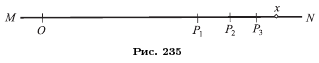
\includegraphics{mppics/ris-235}
\caption{}\label{1938/ris-235}
\end{figure}

Удвоим снова число сторон вписанного шестиугольника, то есть возьмём теперь правильный 12-угольник, найдём его периметр и отложим его на $MN$ от той же точки $O$; 
мы получим тогда отрезок $OP_3$, который будет больше $OP_2$ по той же причине, по какой $OP_2$ больше $OP_1$.

Вообразим, что такой процесс удвоения и откладывания периметров продолжается всё далее и далее.
Тогда мы получим неограниченную последовательность периметров $OP_1, OP_2, OP_3,$ и так далее, которая является возрастающей последовательностью.
Однако возрастание это не может быть неограниченным, так как периметр всякого вписанного многоугольника (выпуклого), каково бы ни было число его сторон, всегда остаётся меньше периметра любого описанного многоугольника (как его объемлющего).
Вследствие этого полученная последовательность периметров правильных вписанных многоугольников имеет определённый предел (§~\ref{1938/229}), обозначенный на чертеже $Ox$.
Этот предел и принимают за длину окружности.

Таким образом, мы принимаем следующее \so{определение}:
\emph{за длину окружности принимается тот предел, к которому стремится (приближается) периметр правильного многоугольника, вписанного в эту окружность, когда число сторон его неограниченно удваивается.}

\smallskip
\so{Замечание}.
Можно доказать (мы опускаем это доказательство), что предел этот не зависит от того, с какого многоугольника мы начинаем удвоение.
Более того, можно доказать, что если даже вписанные многоугольники и не будут правильные, всё же периметры их стремятся к тому же самому пределу, как и периметры правильных многоугольников, лишь бы только стороны их неограниченно уменьшались (и, следовательно, число сторон их неограниченно увеличивалось) путём ли удвоения, как мы это предполагали для правильных многоугольников, или по какому-нибудь иному закону (мы опускаем это доказательство).

 %%%%overfull
Таким образом, для каждой окружности существует свой единственный предел, к которому стремится периметр вписанного выпуклого многоугольника, когда стороны его неограниченно уменьшаются;
предел этот и принимается за длину окружности.

{

\begin{wrapfigure}{r}{41mm}
\centering
\includegraphics{mppics/ris-236}
\caption{}\label{1938/ris-236}
\end{wrapfigure}

Равным образом за длину какой-нибудь дуги окружности $AB$ (рис.~\ref{1938/ris-236}) принимается предел, к которому стремятся длины ломаных линий, вписанных в эту дугу и имеющих с ней одни и те же концы, 
когда их стороны неограниченно уменьшаются.

}

\paragraph{}\label{1938/235}
\so{Лемма}.
\emph{Длина дуги окружности
1) больше стягивающей её хорды, но 2) меньше периметра всякой ломаной линии, описанной около этой дуги и имеющей с ней одни и те же концы} (рис.~\ref{1938/ris-237}).

%??? можно заменить на непревышает и доказательство упроститьсся

\so{Доказательство}.
1) Пусть $ACB$ (рис.~\ref{1938/ris-236}) — дуга окружности и $AB$ — стягивающая её хорда;
требуется доказать, что дуга больше этой хорды.



Предположим, что в дугу мы вписываем правильные ломаные таким образом:
первая ломаная пусть будет составлена из двух хорд $AC$ и $CD$;
вторую ломаную получим путём удвоения числа сторон первой ломаной;
это будет ломаная $ADCEB$, состоящая из четырёх хорд;
третью ломаную получим удвоением числа сторон второй ломаной;
она будет состоять из восьми хорд.
Вообразим, что этот процесс удвоения продолжается неограниченно.
Тогда с каждым удвоением периметр ломаной будет возрастать;
например:
\[AD+DC+CE+EB>AC+CB,\]
так как
\[AD+DC>AC\quad\text{и}\quad CE+EB>CB.\]
Вследствие этого предел, к которому стремятся длины ломаных, должен быть больше длины первой ломаной, то есть больше суммы $AC+CB$, и, значит, должен быть и подавно больше хорды $AB$.
Но предел этот принимается за длину дуги $ACD$, значит, эта дуга больше хорды $AB$.

\begin{wrapfigure}{r}{45mm}
\vskip-4mm
\centering
\includegraphics{mppics/ris-237}
\caption{}\label{1938/ris-237}
\end{wrapfigure}

2) Пусть около дуги описана какая-нибудь ломаная линия (правильная или неправильная — всё равно) (рис.~\ref{1938/ris-237}).
Если концы ломаной совпадают с концами дуги, то эту дугу можно рассматривать как сумму нескольких дуг, из которых каждая объемлется ломаной, состоящей только из двух отрезков.
Пусть одна из таких частей будет дуга $AB$ (рис.~\ref{1938/ris-238}).
Докажем, что длина этой дуги меньше суммы $AC+CB$, которую мы для краткости обозначим одной буквой $S$.
Для доказательства возьмём вспомогательную ломаную $AmnB$, которая получится, если мы срежем угол $C$ каким-нибудь отрезком $mn$, \so{не пересекающимся с дугой} $AB$ (что всегда возможно, если ломаная описана, то есть составлена из касательных).
Обозначим длину этой вспомогательной ломаной $AmnB$ буквой $S_1$.
Так как $mn<mC+Cn$, то $S_1<S$.

\begin{wrapfigure}{r}{45mm}
\centering
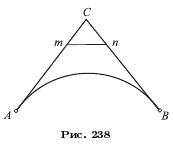
\includegraphics{mppics/ris-238}
\caption{}\label{1938/ris-238}
\end{wrapfigure}

Докажем, что предел, к которому стремятся длины правильных ломаных, вписанной в дугу $AB$, при неограниченном удвоении числа их сторон не может быть больше $S_1$.

Обозначим этот предел буквой $L$ и допустим, что $L>S_1$.
Так как длины ломаных приближается к своему пределу \so{как угодно близко}, то разность между $L$ и такой длиной сделаться меньше разности $L-S_1$; тогда длина такой ломаной сделается больше $S_1$.
Но это невозможно, так как всякая выпуклая ломаная линия, вписанная в дугу $AB$, есть \so{объемлемая} по отношению к объемлющей ломаной $AmnB$ и потому она меньше $S_1$.
Следовательно, нельзя допустить, что $L>S_1$.
Но тогда $L$ должно быть или меньше $S_1$, или в крайнем случае равно $S_1$.
Но так как $S_1<S$, то и в этом и в другом случае должно быть:
$L<S$, что и требуется доказать.

\paragraph{Нахождение длины окружности.}\label{1938/237}
Для этой цели можно пользоваться \so{формулой удвоения}, которую мы вывели раньше (§~\ref{1938/224}), то есть формулой:
\[a_{2n}^2=2R^2-2R\sqrt{R^2-\frac{a_n^2}4}.\]

Если радиус $R$ примем за 1, то формула эта примет более простой вид:
\[a_{2n}^2=2-2\sqrt{1-\frac{a_n^2}4}.\]


Обозначая, по принятому, через $a_n$ сторону правильного вписанного $n$-угольника будем иметь:
$a_6=R=1$.
Применяя формулу удвоения, находим:
\begin{align*}
a_{12}&=2-2\sqrt{1-\tfrac14}=2-\sqrt3;
\\
a_{24}&=2-2\sqrt{1-\tfrac{a_{12}^2}{4}};
\\
a_{48}&=2-2\sqrt{1-\tfrac{a_{24}^2}{4}}\quad\text{и так далее.}
\end{align*}
Положим, что мы прекратили удвоение на 96-угольнике.
Чтобы получить его периметр, надо сторону умножить на 96.
Этот периметр можно принять за приближённое значение длины окружности.
Обозначив его через $p_{96}$ и выполнив вычисления, найдём:
\[p_{96} = 6{,}2820638\dots\]
При радиусе, равном $R$, получим:
\[p_{96}=R\cdot6{,}2820638\dots,
\quad\text{или}\quad
p_{96}=2R\cdot3{,}1410319\dots\]
Обозначая длину окружности буквой $C$, мы получим для неё приближённую формулу:
\[C\approx 2R\cdot3{,}1410319\dots\]
Если бы мы прекратили процесс удвоения на 192-угольнике, то получили бы для длины окружности более точное значение, именно:
\[C\approx2R\cdot3{,}14145247\dots\]
Продолжая процесс удвоения, можно получать для длины окружности всё более и более точные значения.

\paragraph{Отношение длины окружности к диаметру.}\label{1938/238}
Рассматривая процесс нахождения длины окружности, можно заметить, что число, на которое нужно умножить диаметр, чтобы получить длину окружности, не зависит от величины самого диаметра, так что если мы нашли, что длина какой-нибудь окружности равна её диаметру, умноженному на некоторое число, то и длина всякой другой окружности будет равна её диаметру, умноженному на то же самое число.

В самом деле, возьмём две окружности:
одну радиуса $R$, другую радиуса $r$.
Длину первой окружности обозначим через $C$, длину второй — через $c$.
Впишем в каждую из них правильный многоугольник с одним и тем же числом сторон и будем удваивать число сторон каждого из этих многоугольников.

Обозначим через $P_n$ периметр правильного $n$-угольника, вписанного в первую окружность, и через $p_n$ периметр правильного $n$-угольника, вписанного во вторую окружность.

В силу теорем, доказанных в §~\ref{1938/218}, мы можем написать:
\[\frac{P_n}{R}=\frac{p_n}{r}
\quad\text{или}\quad
\frac{P_n}{2R}=\frac{p_n}{2r}.\]

Периметры $P_n$ имеет пределом длину $C$ первой окружности.
Периметры $p_n$ имеет пределом длину $c$ второй окружности.
Значит, из равенства $\frac{P_n}{2R}=\frac{p_n}{2r}$ вытекает
\[\frac{C}{2R}=\frac{c}{2r}.\]
Действительно, поскольку $P_n$ стремится к $C$,
разница $C-P_n$ неограниченно убывает с возрастанием $n$;
а значит и разница
\[\frac{C}{2R}-\frac{P_n}{2R}=\frac{1}{2R}(C-P_n)\]
также неограниченно убывает, то есть последовательность $\frac{P_n}{2R}$ стремится к $\frac{C}{2R}$.
Далее, из равенств $\frac{P_n}{2R}=\frac{p_n}{2r}$,
мы получаем, что последовательность $\frac{p_n}{2r}$ также стремится к $\frac{C}{2R}$.
С другой стороны, эта последовательность должна стремится к $\frac{c}{2r}$ и значит $\frac{C}{2R}=\frac{c}{2r}$.

Таким образом, мы можем сказать, что \emph{отношение длины окружности к её диаметру есть число постоянное для всех окружностей}. 
Это постоянное число принято обозначать греческой буквой $\pi$ (читается «пи»).%
\footnote{Буква $\pi$ есть начальная буква греческого слова \textgreek{περιφέρεια} (окружность).
Обозначение это введено, по всей вероятности, в XVII веке.
}

Мы можем, таким образом, для длины $C$ окружности написать такую формулу:
\[C=2R\cdot\pi
\quad\text{или}\quad
C=2\pi R.
\]
Доказано, что число $\pi$ является числом иррациональным, и, значит, оно не может быть выражено точно никаким рациональным числом.
Но его приближённые значения можно находить различными способами с какой угодно точностью.
Приняв периметр вписанного 96-угольника за приближённую длину окружности, мы получим для $\pi$ приближённое значение $3{,}14$ с недостатком и с точностью до $0{,}01$.
Эта точность для практических целей почти всегда достаточна.
В случаях особенной точности можно довольствоваться таким приближённым значением (с избытком):
$\pi = 3{,}1416$.\footnote{Для запоминания довольно длинного ряда цифр, выражающих число $\pi$, можно пользоваться следующим  двустишием (придуманным покойным преподавателем средней школы Шенроком):
\begin{verse}
Кто и шутя и скоро пожелает(ъ).\\
Пи узнать число уж(ъ) знает(ъ).
\end{verse}
Если выписать в ряд числа букв, заключающихся в каждом слове этих фраз (написанных по старой орфографии), то получим для $\pi$:
приближённое число (с избытком), $3{,}141596536$, верное до одной половины десятибиллионной.}%

Ещё в III веке до нашей эры знаменитый сиракузский геометр Архимед нашёл для $\pi$ очень простое приближение $\tfrac{22}7$ то есть $3\tfrac17$.
Это число несколько более $\pi$ и разнится от него менее чем на 2 тысячных;
оно равно второй подходящей дроби для разложения $\pi$ цепную дробь
\[\pi=3+\frac{1}{7+\frac{1}{15+\frac{1}{1+\cdots}}}.\]
В V веке, китайский математик Цзу Чунчжи нашёл приближение $\tfrac{355}{113}$, это четвёртая подходящая дробь. 
Сейчас вычислены многие триллионы знаков в десятичном разложении $\pi$, что далеко превосходит всякие практические требования.
(Например 40 знаков числа $\pi$ более чем достаточно чтобы вычислить длину окружности радиуса сравнимого с расстоянием до самой далёкой видимой звезды и с точностью превышающей размер атома.) 

При решении геометрических задач часто встречается число, обратное числу $\pi$, то есть равное дроби $\tfrac1\pi$.
Полезно запомнить несколько цифр этого числа.
\[\tfrac1\pi = 0{,}3183098\dots\]

\smallskip
\so{Замечание}.
Число $\pi$ не является рациональным;
более того, оно \so{трансцендентно}, то есть оно не может служить корнем никакого алгебраического уравнения с рациональными коэффициентами.
Это было доказано в 1882 году немецким математиком Фердинандом фон Линдеманом.
В частности, с помощью циркуля и линейки нельзя решить построением задачу о выпрямлении окружности (§~\ref{1938/211}), то есть нельзя построить такой отрезок, длина которого в точности равнялась бы длине данной окружности.


\paragraph{Длина дуги, содержащей $\bm{n}$ градусов.}\label{1938/239}
Длина окружности есть $2\pi R$, значит, длина дуги в $1\degree$ равна $\frac{2\pi R}{360}=\frac{\pi R}{180}$; следовательно, длина $s$ дуги, содержащей $n\degree$, выразится так:
\[s=\frac{\pi R n}{180}.\]
Если дуга выражена в минутах ($n'$) или в секундах ($n''$), то длина её определяется соответственно формулами:
\[s=\frac{\pi R n}{180\cdot 60}
\quad\text{или}\quad
s=\frac{\pi R n}{180\cdot 60\cdot 60},\]
где $n$ — число минут или секунд.

\paragraph{}\label{1938/240}
\so{Задача}.
\emph{Вычислить с точностью до 1 мм радиус такой окружности, дуга которой, содержащая $81\degree 21'36''$, равна $0{,}452$ м.}

Обратив $81\degree 21'36''$ в секунды, получим число 292896.
Из уравнения
\[0{,}452 = \frac{\pi R\cdot  292896}{180\cdot 60\cdot 60}\]
находим:
\[R=\frac{0{,}452\cdot 60\cdot 60}{292896\cdot \pi}=\frac1\pi\approx0{,}318 (\text{м}).\]

\paragraph{}\label{1938/241}
\so{Задача}.
\emph{Определить число градусов дуги, длина которой равна радиусу.}

Заменив в формуле, определяющей длину дуги в $n\degree$, величину $s$ на $R$, получим уравнение:
\[R=\frac{\pi R n}{180}
\quad\text{или}\quad
1=\frac{\pi n}{180}\]
откуда
\[n\degree = 180\degree \cdot \frac1\pi \approx 180\degree \cdot 0{,}3183098 = 57{,}295764\degree \approx 57\degree17'44''\]

\paragraph{Радианы.}\label{extra/radians}
Дуга, равная радиусу, называется \rindex{радиан}\textbf{радианом}.
В радианах принято мерить и углы — за угол в один радиан берут центральный угол который вырезает из окружности дугу равную её радиусу.

Радианы считаются за основную единицу измерения углов --- если единица измерения углов не указывается, то всегда имеется ввиду радиан.
Например, прямой угол это «угол равный $\tfrac\pi2$», развёрнутый угол --- «угол равный $\pi$».
Градус это второстепенная единица удобная для работы с дробными частями прямого угла;
$1\degree =\tfrac\pi{180}\approx 0{,01745}$.

Заметим, что если $\alpha$ есть угловая величина дуги $AB$ окружности радиуса $R$ выраженная в радианах то её длину можно выразить формулой
\[s=\alpha\cdot R.\]
Аналогичная формула для угла измеренного в градусах (§~\ref{1938/239}) существенно сложнее.
%!!!добавил замечание

\subsection*{Упражнения}

\begin{enumerate}

\item
Доказать, что в двух кругах отношение центральных углов, соответствующих дугам, имеющим одинаковую длину, равно обратному отношению радиусов.

\item
На окружности взята точка $A$ и через неё проведены:
диаметр $AB$, сторона правильного вписанного шестиугольника $AC$ и касательная $MN$.
Из центра $O$ опущен на $AC$ перпендикуляр и продолжен до пересечения с касательной в точке $D$.
От этой точки отложен по касательной (через точку $A$) отрезок $BE$, равный трём радиусам.
Точка $E$ соединена с концом диаметра $B$.
Определить, как велика погрешность, если прямую $BE$ возьмём за длину полуокружности.

\item
На диаметре данной полуокружности построены две равные полуокружности, и в ту часть плоскости, которая заключена между тремя полуокружностями, вписан круг.
Доказать, что диаметр этого круга относится к диаметру равных полуокружностей, как $2:3$.

\item
Вычислить в градусах, минутах и секундах дугу, равную стороне квадрата, вписанного в эту окружность.

\item
Вычислить длину $1\degree$ земного экватора, принимая радиус Земли равным 6400 км.

\end{enumerate}